% Author: Joshua Carey

%
\let\textcircled=\pgftextcircled
\chapter{Methodology}
\label{chap:aims_and_opjectives}

\initial{T}his section will investigate the approach taken to create an autonomous kite-powered vessel.
- We need a physics engine
-we need to model a boat so that it behaves with realistic movements
- need to be able to run machine learning in the physics simulations

\section{A Simulation Environment}
In the endeavor to establish a robust and realistic simulation environment, that would act as that platform for training a reinforcement learning model, an appropriate simulation environment had to be chosen.  

\section{Training Environment}
Unity has a comprehensive physics engine built in, it allows for easy creation of mesh bodies and colliders, rigid bodies and configurable joints. These would all come in very handy in while trying to model the complex system of a kite-boat, significantly reducing the development time while still maintaining a complex and realistic system. Another feature of the game engine that became the starting point for the physics model was the Unity HDRP Water System 16.0.3 [cite], that is available in the latest beta version Unity 2023.2.0b9 [cite]. The first steps to creating a comprehensive model ready for training is to model Buoyancy and a rudder, making a controllable playable boat.

\subsection{Buoyancy}
To model buoyancy accurately, first the maths had to be reviewed. When a body is submerged in a fluid the fluid exerts a force on the surface of the body, due to the pressure in the fluid. Archimedes Principal states that "The upward buoyant force that is exerted on a body immersed in a fluid, whether partially or fully submerged, is equal to the weight of the fluid that the body displaces and acts in the upward direction at the center of mass of the displaced fluid", shown in equation \ref{archimedes}. In order to model the buoyancy of a complex object, such as a boat hull, the 'amount' of boat below the water needed to be calculated. In Unity the boat hull was a 'mesh' with a 'mesh collider' attached to it, this was incredibly helpful as it takes on the complex challenge of splitting the surface of the hull into many small triangles or Voxels 

\begin{equation}
    F_B = \rho_{w}gV
    \label{archimedes}
\end{equation}

The total Archimedes force (AF) of the entire boat was calculated using equation \ref{archimedes}, followed by a local AF at each Voxel. The water level, y component, was then computed at each voxel's (x,z) coordinates to determine if it was above or below the surface. If below the surface the component of the AF was applied vertically at each voxel. 

\subsection{Rudder}
The rudder was created as a rigid body and modeled as a simple symmetric foil using the force diagram in figure \ref{rudderForce}. The lift and drag forces were calculated using equations \ref{lift} and \ref{drag}, where ${C_l}$ is the lift coefficient, ${C_d}$ is the drag coefficient, A is the sing surface area, V is the velocity of the water and ${\rho}$ is the density of the water.



\begin{equation}
    L = {C_l}A\rho\frac{V^2}{2}
    \label{lift}
\end{equation}
\begin{equation}
    D = {C_d}A\rho\frac{V^2}{2}
    \label{drag}
\end{equation}
 
\begin{figure}
    \centering
    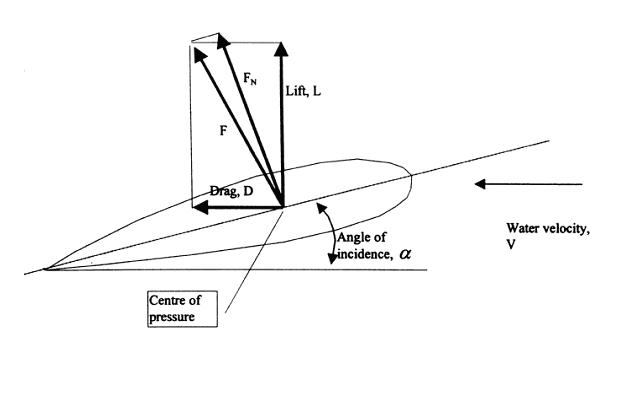
\includegraphics{chapters/chapter04/rudder.JPG}
    \caption{Force Diagram of a boat rudder}
    \label{rudderForce}
\end{figure}

\subsection{Course Generation}

\subsection{Mark Roundings}

\section{MLAgents}

\section{The Boat Agent}

\section{Initial Training}

\section{Optimization}

%=======
\label{sec:sec01}





%=========================================================